\documentclass{article} % For LaTeX2e
\usepackage{nips15submit_e,times}
\usepackage{hyperref}
\usepackage{url}
\usepackage{graphicx}
%\documentstyle[nips14submit_09,times,art10]{article} % For LaTeX 2.09


\title{Multi-scale Human Detail Restoration}


\author{
Chu Chu \\
Department of Computer Science\\
Simon Fraser University\\
8888 University Dr, Burnaby, BC V5A 1S6 \\
\texttt{chuc@sfu.ca} \\
\And
Shitao Tang \\
Department of Computer Science\\
Simon Fraser University\\
8888 University Dr, Burnaby, BC V5A 1S6 \\
\texttt{shitaot@sfu.ca} \\
}

% The \author macro works with any number of authors. There are two commands
% used to separate the names and addresses of multiple authors: \And and \AND.
%
% Using \And between authors leaves it to \LaTeX{} to determine where to break
% the lines. Using \AND forces a linebreak at that point. So, if \LaTeX{}
% puts 3 of 4 authors names on the first line, and the last on the second
% line, try using \AND instead of \And before the third author name.

\newcommand{\fix}{\marginpar{FIX}}
\newcommand{\new}{\marginpar{NEW}}

\nipsfinalcopy % Uncomment for camera-ready version

\begin{document}


\maketitle

\begin{abstract}
Recent development of deep learning has made it possible to reconstruct  human from a single RGB image. However, most existing approaches can only restore a general shape without details on body, e.g. clothes wrinkles. Among those methods, one of the most important steps is to estimate depths from RGB images. Most approaches treat the human depth estimation as a regression problem. We conjure that it is difficult for convolutional neural network to predict the depth image directly. Instead, we propose to learn the depths in a coarse-to-fine manner. We first build both the Laplacian pyramids of depth images and the feature pyramid of ConvNets at different scales. The Laplacian pyramids is used to guide the learning of feature pyramids. The initial experiments show that our approach is a promising  direction for human detail restoration.
\end{abstract}

\section{Introduction}
Reconstructing 3D models from RGB images has been studied since the concept of artificial intelligence was proposed. Current traditional methods, such as multiview-stereo, structure-from-motion, shape-from-texture, are successful to reconstruct the general shape of objects, e.g. cups, chairs, desks, but these methods typically require the objects, of which there are multiple RGB images available, to be simple. In contrast, when dealing with complex objects, typically humans, traditional geometry-based methods can only generate overall shape and fail to restore the details on the shape, e.g. clothes wrinkles~\cite{izadi2011kinectfusion,wu2017marrnet,newell2016stacked,li2015maximum,toshev2014deeppose}. One of the biggest challenges is that rich and robust features, which these methods rely on, are difficult to be captured by hand-crafted feature extractors. In addition, since a single image can hardly provide geometry constraints, rarely methods can do 3D reconstruction using one single RGB image.

Recent researches on learning-based methods, especially convolutional neural network (CNN), has demonstrated its powerful feature extraction ability.~\cite{he2016deep,simonyan2014very} As a result, many works have adopted CNN to generate 3D models of humans from a single image without using geometry constraints~\cite{tang2019neural,fan2017point}, which is superior than traditional methods requiring multiple images. Learning-based methods generally train a CNN in a large dataset of scanned body shapes.~\cite{tang2019neural} While generating 3D models, these methods only inference the naked body shape without capturing the clothes details. 

Tang et al.\cite{tang2019neural} is the first work to recover a detailed depth map for the foreground human object from a single RGB image. This paper proposes to separate the depth into a smooth base shape and a residual detail shape, and regress them respectively. The base shape captures the large overall geometry layout, while the detail shape captures small bumps such as cloth wrinkles. The value range of the base shape is at the scale of one meter, while the detail shape is at a few centimeters. One of limitations of this work is that both the base branch and detail branch use the same feature map, which prevent the base branch learning a coarse overall shape. We argue that the base (coarse) shapes are low-frequency signals while the details are high-frequency signals so they should be better predicted by feature maps at different scales.

%that should be better predicted by larger fine feature maps. that should be better predicted by the final feature map whose receptive field is largest,
Lin et al.~\cite{lin2017feature} proposes feature pyramid network (FPN) to detect objects at different scales. FPN computes a feature hierarchy layer by layer, and with sub-sampling layers, the feature hierarchy has an inherent multi-scale, pyramidal shape. This in-network feature hierarchy produces feature maps of different spatial resolutions without introducing large semantic gaps caused by different depths since the bottom features and top features are connected through up-sampling.

Inspired by those works, we propose to build both depth image pyramid and feature pyramid. The image pyramid guides the learning of the feature pyramid. For image pyramid, top images contain the coarsest shapes, bottom images contain the finest details and middle images are in between. Each image in the image pyramid guides the learning of each feature map in pyramid of CNN in a one-to-one manner. The coarsest image is predicted by the top feature map since its receptive field is the largest and the finest image is predicted by the bottom feature since its spatial size is largest and contains more detailed information.



%% \subsection{Double-blind reviewing}

%% This year we are doing double-blind reviewing: the reviewers will not know 
%% who the authors of the paper are. For submission, the NIPS style file will 
%% automatically anonymize the author list at the beginning of the paper.

%% Please write your paper in such a way to preserve anonymity. Refer to
%% previous work by the author(s) in the third person, rather than first
%% person. Do not provide Web links to supporting material at an identifiable
%% web site.

%%\subsection{Electronic submission}
%%
%% \textbf{THE SUBMISSION DEADLINE IS June 5, 2015. SUBMISSIONS MUST BE LOGGED BY
%% 23:00, June 5, 2015, UNIVERSAL TIME}

%% You must enter your submission in the electronic submission form available at
%% the NIPS website listed above. You will be asked to enter paper title, name of
%% all authors, keyword(s), and data about the contact
%% author (name, full address, telephone, fax, and email). You will need to
%% upload an electronic (postscript or pdf) version of your paper.

%% You can upload more than one version of your paper, until the
%% submission deadline. We strongly recommended uploading your paper in
%% advance of the deadline, so you can avoid last-minute server congestion.
%%
%% Note that your submission is only valid if you get an e-mail
%% confirmation from the server. If you do not get such an e-mail, please
%% try uploading again. 


\subsection{Related Work}
\textbf{Body Shape Estimation.} The 3D shape of the human body can be parameterized by the SCAPE or SMPL models with two sets of independent parameters, controlling the skeleton pose and body shape respectively. Both models are derived from a large set of scanned 3D human shapes. Given these parametric human models, many methods recover dense human body shape from a single RGB image by estimating the shape and pose parameters. Meanwhile, there are also some non-paramterized methods which directly regress discretized body shape representation from an RGB image. The above methods only recover the 3D shape of the naked human body, however, geometry details like the clothes are not modeled, which make them not suitable for visualization tasks. While the method can predict the SMPL model with clothe wrinkles, it needs to be fed a video of a moving person with designed pose. Tang et al.~\cite{tang2019neural} proposes a neural network to reconstruct 3D human model. The whole framework contains the skeleton-net and segmentation-net,which generates the heatmaps of 3D skeleton joints and body part segmentation respectively. Then, their results are further fused with the input image to compute the base shape and detail shape via the depth-net. In a separate branch, the normal-net estimates a fused in the depth refinement module to produce the final result. Our method avoid the use of segmentation-net, skeleton-net and normal-net but only optimize depth-net to generate detailed human models.

\textbf{Generic Dense Depth Estimation.} Depth estimation from a single image has gained increasing attention in the computer vision community. Most works are proposed for indoor and outdoor scenes. Godard et al.~\cite{godard2017unsupervised} proposes an unsupervised method that train a CNN to estimate depths from a single RGB image with left-right consistency. However, this method requires paired images of the same scene, limiting its usage in practice. Eigen et al.~\cite{eigen2014depth} applies multi-scale networks which stage-wisely refine estimated depth map from low spatial resolution to high spatial resolution via independent networks. However this method adopts two different networks to propose images at different scales, which adds addition computation cost. Our work aims at developing an end-to-end network that takes a single RGB image as input and outputs the depth image as result.

\textbf{Object Detection.} The rapid development of deep learning has boost the performance of object detection to an unprecedented level. One of challenges is how to detect objects at different scales. Feature pyramid networks (FPN)~\cite{lin2017feature} computes a feature hierarchy layer by layer. With sub-sampling layers, the feature hierarchy has an inherent multi-scale, pyramidal shape and combines low-resolution, semantically strong features with high-resolution, semantically weak features via a top-down pathway and lateral connections. Our work directly follows the same design spirit and adopts its basic architecture as our backbone. 
\begin{figure}
    \centering
    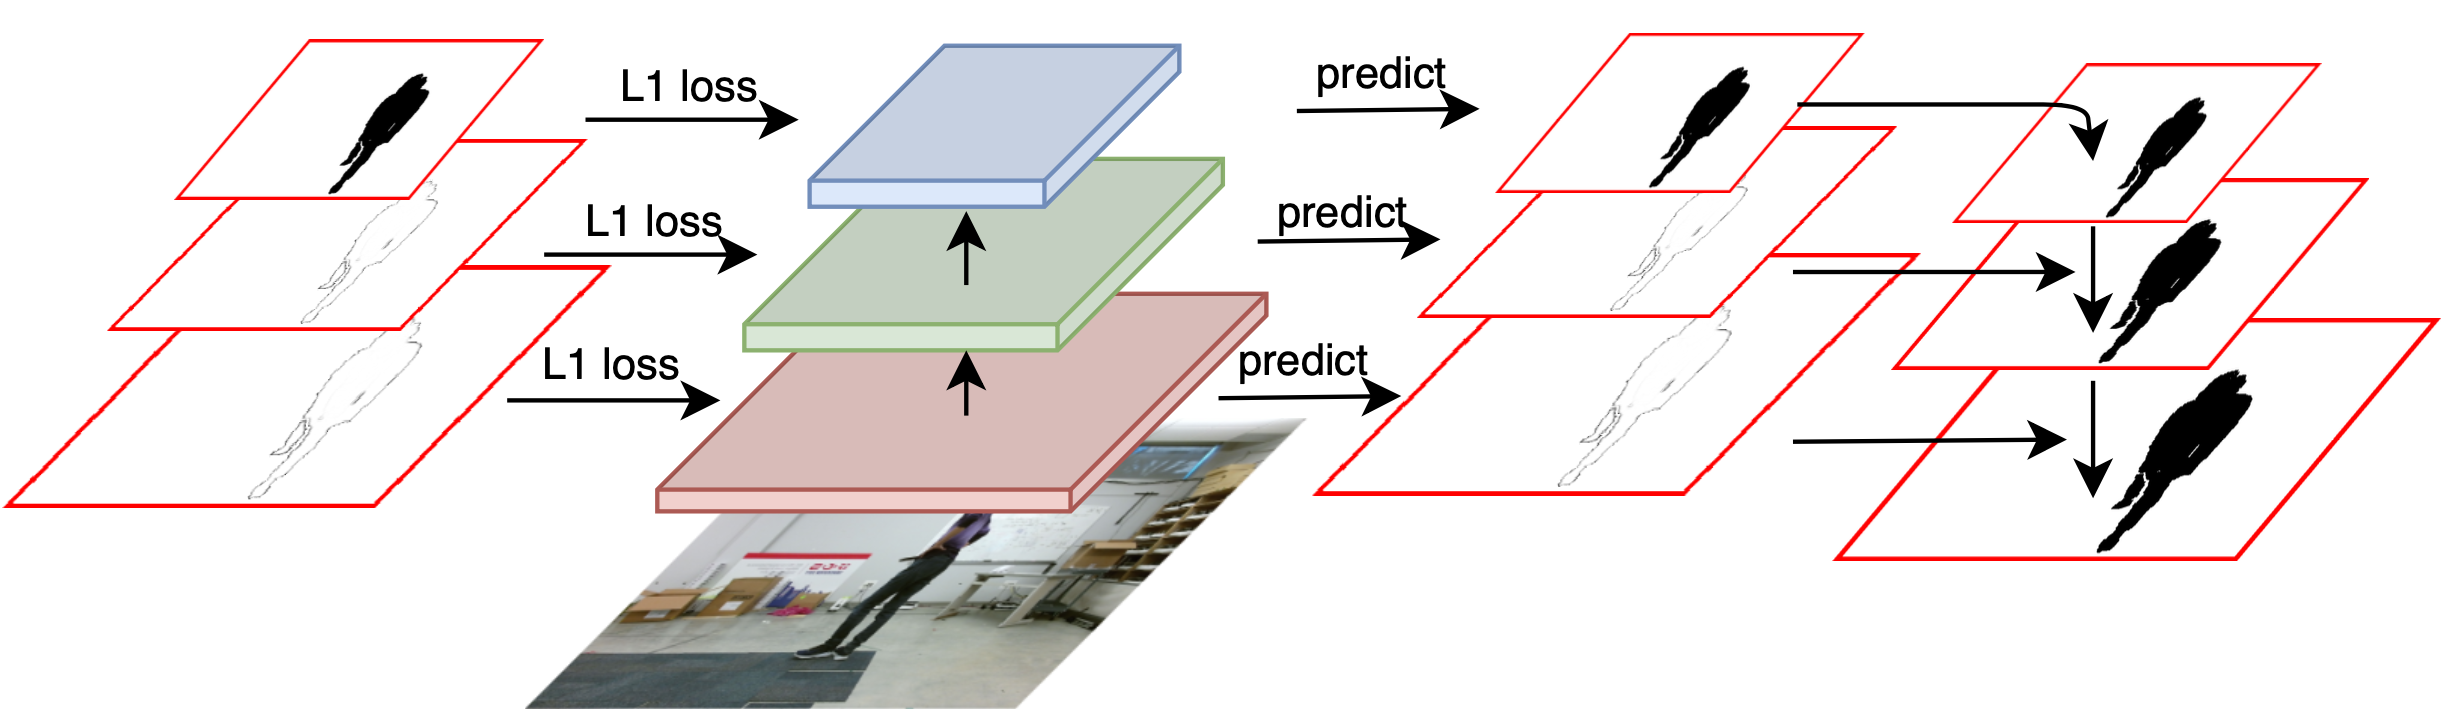
\includegraphics[width=\textwidth]{pipeline.png}
    \caption{Illustration of our methods. We build the laplacian depth image pyramid and the feature pyramid. The image pyramid guides the learning of feature pyramid.}
    \label{fig1}
\end{figure}
\section{Methods}
As illustrated in Fig.\ref{fig1}, our model takes in a single RGB image and the feature map is supervised by the laplacian depth images hierarchically. In the inference stage, the predictions are summed to form the final depth map. In the following sections, we introduce the laplacian depth image pyramid, the feature pyramid and the loss function.

\subsection{Laplacian Depth Image Pyramid}
The separate predictions of base shapes and detailed shapes proposed by Tang et at.\cite{tang2019neural} has been proved to be successful. The base shapes are obtained by applying the bilateral filter to the depth images while the detailed shapes are residuals between the original images and the depth images. The bilateral filter is a non-linear, edge-preserving, and noise-reducing smoothing filter for images. It replaces the intensity of each pixel with a weighted average of intensity values from nearby pixels. Therefore, the images, as shown in Fig.\ref{fig2}, are blurred after applying the filter. For the detailed images (residuals), it keeps the lines and eliminates blocks of constant colors. These two depth images are predicted by two different branches without sharing parameters, which can be better optimized since they can focus on different patterns. 

\textbf{Gaussian image pyramid.} As shown in Fig.\ref{fig2}, Gaussian image pyramid is a set of images of different resolutions. The original image is repeatedly filtered (typically bilateral filter) and sub-sampled to generate the sequence of reduced resolution images. These comprise a set of lowpass filtered copies of the original image in which the bandwidth decreases in one octave step. The bottom is the origin image and the top is the lowest-resolution image. The resolution of i-th layer is $(\frac{1}{2})^i$. 

\textbf{Laplacian image pyramid.} As shown in Fig.\ref{fig2}, Laplacian image pyramid is similar to Gaussian image pyramid but saves difference images in Gaussian pyramid between each level. The smallest level is the same as the one in Gaussian pyramid instead of a difference image, which enables reconstruction of the high resolution image using the difference images on higher levels. The original image can be reconstructed by first up-sampling the images to the same resolution and them summing them. The different images are easy to predicted since the model do not need to predict the featureless areas. In ~\cite{tang2019neural}, the base shape and the detailed shape form a 2-layer Laplacian image pyramid. Our method uses 3-layer Laplacian depth image pyramid, denoted by $\{D_1, D_2, D_3\}$, which allows the network to recover more detailed regions. 

\begin{figure}
    \centering
    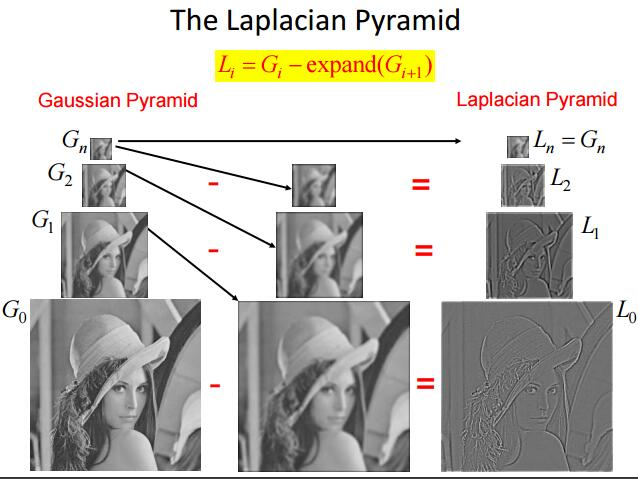
\includegraphics[width=\textwidth]{the-laplacian-pyramid.jpg}
    \caption{Illustration of Gaussian pyramid and Laplacian pyramid.~\cite{pyramid}}
    \label{fig2}
\end{figure}

\subsection{Feature Pyramid}
Our method adopts the feature pyramid network~\cite{lin2017feature} as backbone, takes a single-scale image of an arbitrary size as input, and outputs proportionally sized feature maps at multiple levels, in a fully convolutional fashion. The construction of feature pyramid involves a bottom-up pathway, a top-down pathway, and lateral connections, as introduced in the following.

\textbf{Bottom-up pathway.} The bottom-up pathway is the feed-forward computation of the backbone ConvNet, which computes a feature hierarchy consisting of feature maps at different scales with a stride of 2. Taking ResNets~\cite{he2016deep} as example, the feature activation's output by each stage’s last residual block are used. We denote the output of these last residual blocks as $\{C_1, C_2, C_3, C_4\}$ for conv2, conv3, conv4, and conv5 outputs, and note that they have strides of $\{4, 8, 16, 32\}$ pixels with respect to the input image.

\textbf{Top-down pathway.} The top-down pathway forms higher resolution features by upsampling operation, but semantically stronger. These features are enhanced with features from the bottom-up pathway via lateral connections. Each lateral connection merges feature maps of the same spatial size from the bottom-up pathway and the top-down pathway. The bottom-up feature map is of lower-level semantics, but its activations are more accurately localized as it was subsampled fewer times. FPN upsamples the spatial resolution by a factor of 2. The upsampled map is merged with the corresponding bottom-up map (which is applied by a 1*1 convolutional layer to reduce channel dimensions) by element-wise addition. This process is iterated until the finest resolution map is generated. To start the iteration, we simply attach a 1*1 convolutional layer on the top feature to produce the coarsest resolution map. Finally, we append a 3*3 convolution on each merged map to generate the final feature map, which is to reduce the aliasing effect of upsampling. This final set of feature maps is called $\{P_2, P_3, P_4, P_5\}$, corresponding to $\{C_1, C_2, C_3, C_4\}$ that are respectively of the same spatial sizes. Note that the operations are the same as the one used to reconstruct images in the Laplacian image pyramid. We only use $\{C_1, C_2, C_3\}$ in our methods since 3-layer pyramid has reached satisfactory performance.

\subsection{Training and Inference}
\textbf{Training.} We map Laplacian image pyramid $\{D_1, D_2, D_3\}$ to feature pyramid $\{P_1, P_2, P_3\}$ and use $P_n$ to predict $D_n$. The size of $\{P_1, P_2, P_3\}$ is the same as $\{D_1, D_2, D_3\}$ since they are both down-sample by the same steps. As for the loss function, for simplicity, we only try the following L1 loss.
\begin{equation}
    L=\frac{1}{n}\sum_i^n |p_i-d_i|
\end{equation}
where $n$ is the total number of pixels of the image pyramid, $p_n$ and $d_i$ are the predictions and pixel values in the same location. 

\textbf{Inference.} In inference stage, we can construct the predicted depth image by summing and upsampling the prediction, $\{P_1,P_2,P_3\}$ as the same construction procedure of restoring the original image by the Laplacian image pyramid.

\section{Experiment}\label{exp}
To illustrate the effectiveness of our method, we do evaluation quantitatively.

\textbf{Dataset.} The dataset we used are named PersonDepth, in \cite{tang2019neural}, where there are 26 different people performing simple actions. The dataset is collected by a Microsoft Kinect2 camera. For the training data, there are about 20,000 training depth images in total, 800 frames for each person. For quantitative evaluation, depth cameras are used to capture video clips of a person with a fixed pose and the InfiniTAM~\cite{kahler2015very} are adopted to fuse captured sequences. The high-quality depth maps are rendered according to the fused mesh and camera poses with Blender~\cite{blender2014blender}. The testing data contains 5 different persons, each person is captured with 12 different poses and 3 different clothing styles.

\textbf{Evaluatio metric.}For quantitative evaluation, we use Mean Absolute Error (MAE) as the only metric to evaluate our methods, which is calculated by the mean of absolute value of difference between predictions and ground truths.

\textbf{Training details.}We implement our method using Pytorch~\cite{paszke2019pytorch}. We choose ResNet-18 as our backbone and remove the top basic block to make it efficient. 20000 images in PersonDepth are used to train our model and evaluate it on the testing set. We use adam to optimize the network with an initial learning rate of $1e-5$.  The weight decay is set to $1e-4$. The network is trained for 10 epochs in a single GPU. We use ImageNet~\cite{deng2009imagenet} to pretrain the model and freeze all the batch normalization layer(All the parameters in BN are not updated).

\begin{table}[]
    \centering
    \begin{tabular}{c|c}
    \hline
        Methods & MAE (cm) \\
    \hline
        DR & 10.09 \\
    \hline
        TSR & 10.00 \\
    \hline
        MSR (ours) & 9.92 \\
    \hline
    \end{tabular}
    \caption{Results of different methods in terms of MAE (centimeters) in PersonDepth. DR means directly regressing the depth values using features $p_1$. TSR means two stage regression used in \cite{tang2019neural} with the same features $P_1$. MSR means multi-scale regression proposed in this paper.}
    \label{table1}
\end{table}
\subsection{Results}
We mainly compare three methods and implement them in a single unified Pytorch framework. As shown in table.\ref{table1}, DR is to directly regress the per-pixel depth values on features $P_1$. TSR means two-stage regression used in the original paper~\cite{tang2019neural}, which regress both base shape and detailed shape using the same features $P_1$. MSR means multi-scale regression proposed in this paper, which use  $P_1,P_2,P_3$ to regress details at different scales. Both models adopt the same training procedure explained in Sec.\ref{exp}. We can see that DR reaches an error of 10.09, TSR reaches 10.00 while our methods reaches 9.92, which outperforms the other methods marginally. The improvement is not very significant since we don't have much time to fine-tune the hyper-parameters. However, it suggest predicting depths at different scales is a promising direction for human details restoration. 

\section{Conclusion and Future Work}
We present a method for estimating human depth in a coarse-to-fine manner. We first build a 3-layer laplacian depth image pyramid. The network takes in a single RGB image and outputs 3 different feature maps at different scales with the same size of the corresponding depth image in the lapacian image pyramid. In the training stage, the pyramid serves as ground truth to guide the learning of feature maps. In the inference stage, the predictions at different scales are up-sampled and summed together to get the final depth images. The experiment results show that current approach can only improve the performance marginally, which indicates that there is still room to make improvement. 

Firstly, we use L1 loss to train all three feature maps, but we conjure that it is not suitable for the base shape prediction since both the absolute value and the variance of the top depth image in the Laplacian image pyramid are the largest. The network would try to fit each ground truths perfectly if using L1 loss (small error has large gradients), increasing the learning difficult. As suggested in ~\cite{tang2019neural}, the value of base shape are grouped into several bins and treated as classification, which reduces the prediction space and facilitate the learning. We plan to adopt the strategy or use smooth L1 loss~\cite{girshick2014rich} in the future, which has lower errors than L1 loss when the predictions are close to the ground truths.

Secondly, Laplacian image pyramid may not be the best for image pyramid construction. As shown in Fig.\ref{fig2}, the top image has positive depth values across all the region while the others only have positive ones near line regions. They are two different types of images while the feature pyramid are semantically equivalent. In order to make them more similar, the top image could be made coarser so that the bottom images could have more regions with positive depth values.

To sum up, this paper presents a basic idea towards human depths restoration and the initial attempt shows promising results. However, our approach is still rudimentary and there are a lot of works to be done in the future.

\appendix
\section{Contributions}
Chu and Shitao contribute equally to this paper. Shitao came up with rudimentary idea and Chu helped to refine it. Chu and Shitao both wrote the codes and the paper together.
\bibliographystyle{unsrt}
\bibliography{ref}
\end{document}
